\section{METHODS PIPELINES}
\label{METHODS PIPELINES}
\subsection{Raw data}
Example of the MFL data is shown in Fig.~\ref{ris:data_example}.

\begin{figure}[ht]
	\center{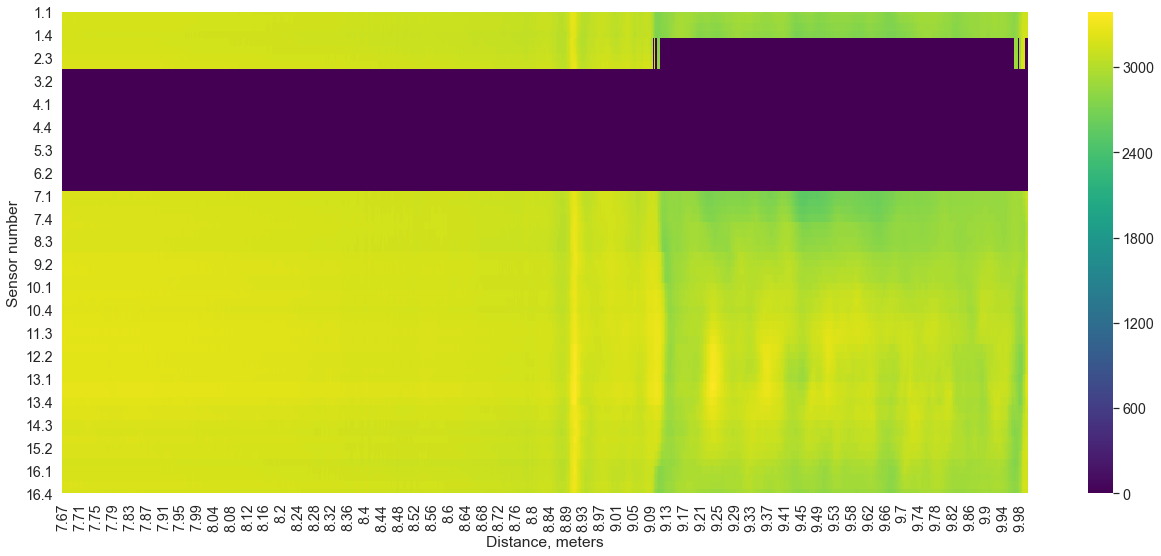
\includegraphics[scale=0.3]{pictures/0.png}}
	\caption{Example of the MFL data}
	\label{ris:data_example}
\end{figure}
Each MFL dataset provides information about single inspection tool run.
Selected for the research dataset represents 15162.85 meters length pipeline part.
It has 745 defects of different types and 1462 welds.
Fig.~\ref{ris:defect_example} shows examples of normal data, data with the weld and defect.
Attached to the dataset technical report contains information about welds and defects location, defects types and sizes and other related data.
\begin{figure}[ht]
	\center{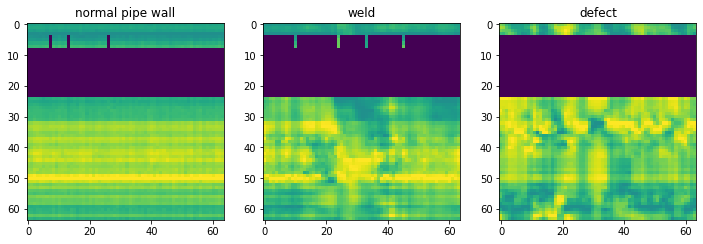
\includegraphics[scale=0.55]{pictures/1.png}}
	\caption{Example of the MFL data}
	\label{ris:defect_example}
\end{figure}

Raw data has several issues that don't allow to solve CV problems without proper preprocessing.
They are:
\begin{enumerate}
	\item Sensors malfunctions (zeroed values cause bold horizontal line in Fig.~\ref{ris:data_example});
	\item Displaced origins between data and report files coordinates;
	\item Inaccurate annotations, e.g. missed defect, wrong defect location, etc.
\end{enumerate}

In addition to preprocessing, data were annotated for the segmentation task.

\subsubsection{Sensors malfunctions problem}
To deal with sensors malfunctions we suppose to fill the gaps (zeroed values) with values calculated by different methods:
\begin{enumerate}
	\item Scaling of picture values to $[0.5:1]$ range. Abnormal values ($<2000$) are equal to 0.
	\item Abnormal values are equal to the mean of normal values from one picture.
	\item Abnormal values are equal to the mean of normal values over the column.
	\item Abnormal values are equal to the mean of neighboring sensors over the column.
	\item Abnormal values are equal to the interpolation results over the column.
	\item Replacing Abnormal values to NaN and rerange in accordance  skimage procedure 
	\item Rerange initial set of values to 0...255 uint8 range.
	\item Rerange initial set of values to 0...1 float range.
	
	
\end{enumerate}
The results of all applied methods are presented in Fig.~\ref{ris:filling_example}.
\begin{figure}[ht]
	\center{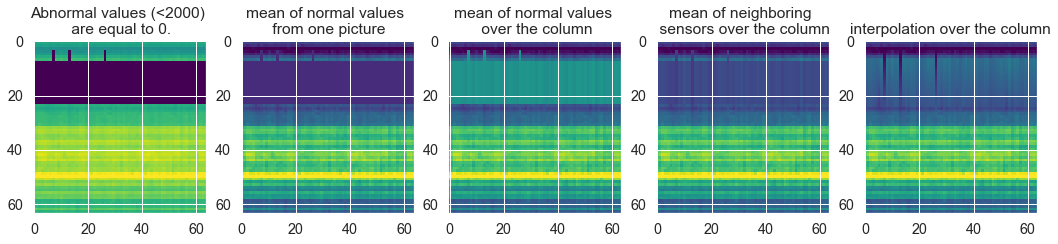
\includegraphics[scale=0.4]{pictures/2.png}}
	\caption{The results of missing values filling methods}
	\label{ris:filling_example}
\end{figure}

\subsubsection{Displaced origins problem}

Since the data on the location of the robot did not match the defect location data from the report, it was necessary to merge the data. The key factor here turned out to be that the values of signal from magnetic flux sensors grow at the weld site, see picture \ref{ris:prepr}. 

\begin{figure}[!h]
	\center{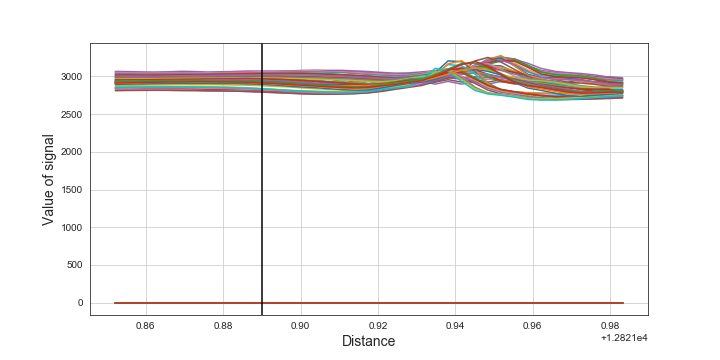
\includegraphics[width=0.7\linewidth]{pictures/prepr.png}}
	\caption{Location of weld. Black vertical line in accordance with defect location data from the report. Others lines are values from sensors.}
	\label{ris:prepr}
\end{figure}
The locations of maxima of these values have been founded and then combined with welds locations.


\subsubsection{Inaccurate annotations problem}


\subsection{Augmentation}
Although we have a lot of data, we don't have a lot of defects and welds in comparison with normal pipe wall instances.
We use augmentation procedure to balance classes of pictures and increase model's quality by increasing number of instances in small classes (defects, welds).
As an augmentation tool we use Albumentations library \cite{buslaev2020albumentations}.
For welds pictures we apply following augmentations:
\begin{enumerate}
	\item Rotate (limit=180, p=1),
	\item VerticalFlip (p=1), 
	\item HorizontalFlip (p=1), 
	\item ElasticTransform (p=1, alpha=20, sigma=120 * 0.05, alpha affine=120 * 0.03), 
	\item GridDistortion (p=1),
	\item OpticalDistortion (p=1, distort limit=2, shift limit=0.5),
\end{enumerate}

And for defects we apply following ones:
\begin{enumerate}
	\item Rotate (limit=180, p=1),
	\item VerticalFlip (p=1), 
	\item HorizontalFlip (p=1), 
	\item ElasticTransform (p=1, alpha=20, sigma=120 * 0.05, alpha affine=120 * 0.03), 
	\item GridDistortion (p=1),
	\item OpticalDistortion (p=1, distort limit=2, shift limit=0.5),
\end{enumerate}
Examples of augmentations are shown in Fig.~\ref{ris:aug_example}.
\begin{figure}[ht]
	\center{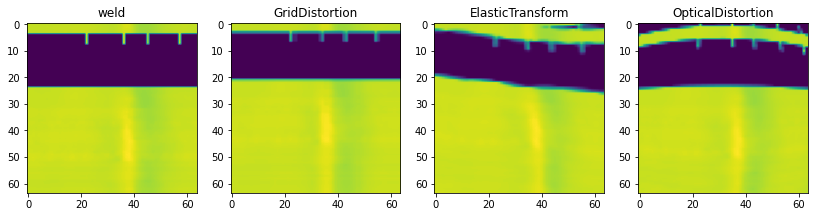
\includegraphics[scale=0.55]{pictures/4.png}}
	\caption{Example of the MFL data}
	\label{ris:aug_example}
\end{figure}


\begin{table}[!htb]
	\caption{\label{tab:alg1}Dataset size for pipeline defects detection problem}
	\begin{center}
		\small
		\begin{tabular}{| l | c | c |}
			\hline
			Class name & train & test \\
			\hline
			\multicolumn{3}{|c|}{Before augmentation}  \\
			\hline
			Normal pipe wall  & 11106 & 584 \\
			Defect & 1130 & 282 \\
			Weld & 569 & 142 \\
			\hline
			\multicolumn{3}{|c|}{After augmentation}  \\
			\hline
			Normal pipe wall & 11106 & 584 \\
			Defect & 8897 & 282 \\
			Weld & 7680 & 142 \\
			\hline
		\end{tabular}
	\end{center}
\end{table}

